\documentclass[tikz,border=12pt]{standalone}
\usepackage[T1]{fontenc}
\usepackage{mathpazo}
\usepackage{amsmath,amssymb}
\usetikzlibrary{arrows.meta, positioning, calc}

\definecolor{stblue}{HTML}{7B97AD}
\definecolor{rwgold}{HTML}{B8995E}
\definecolor{sage}{HTML}{7A9A7E}
\definecolor{dkbrown}{HTML}{3D3530}
\definecolor{wmgray}{HTML}{7B7067}
\definecolor{cream}{HTML}{F9F6F0}
\definecolor{border}{HTML}{D4C9B8}

\begin{document}
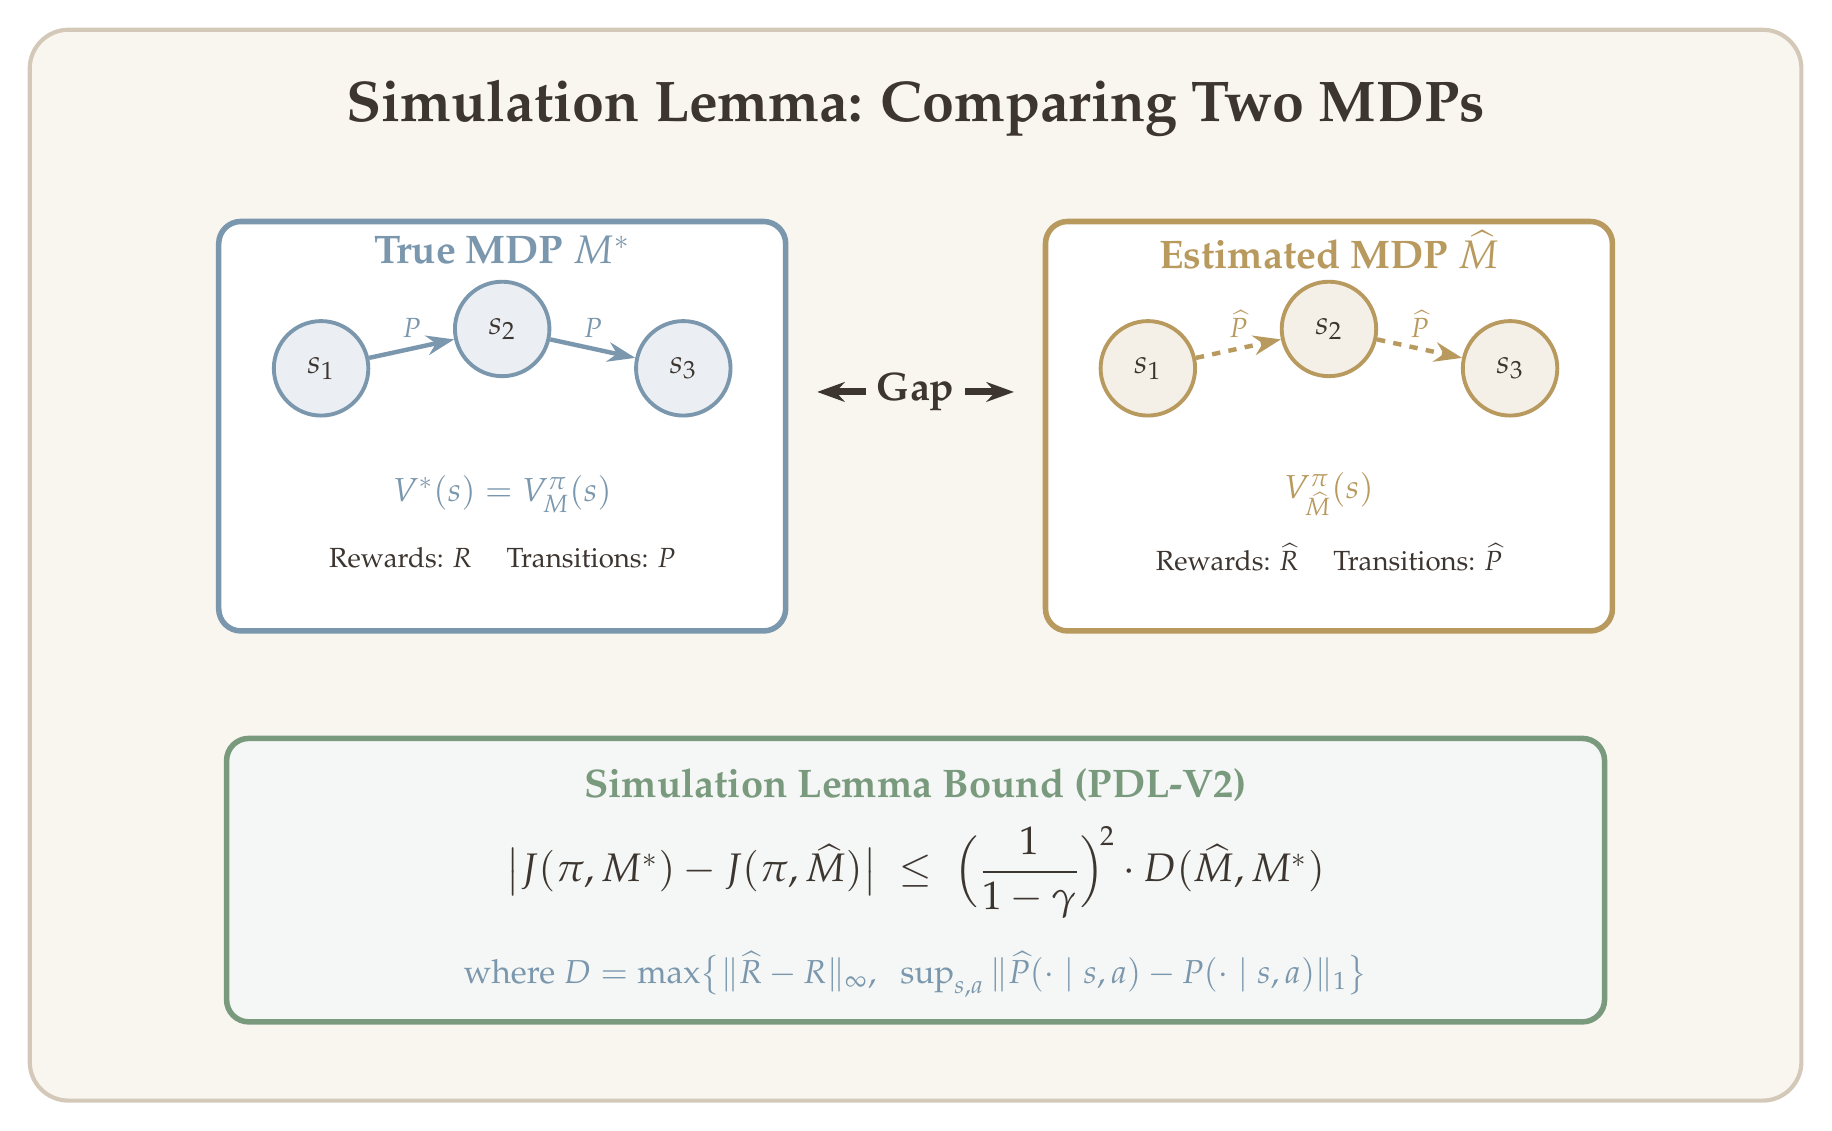
\begin{tikzpicture}[
  >={Stealth[length=3.5mm, width=2.5mm]},
  mdpbox/.style={draw=#1, line width=2pt, fill=white, rounded corners=8pt,
    minimum width=72mm, minimum height=52mm, anchor=north},
  statecircle/.style={circle, draw=#1, line width=1.4pt, fill=#1!15,
    minimum size=12mm, font=\large, text=dkbrown, inner sep=0pt},
  arr/.style={->, line width=1.6pt, dkbrown},
]

% Background
\fill[cream, rounded corners=14pt] (-1.5,-7.8) rectangle (21.0,5.8);
\draw[border, rounded corners=14pt, line width=1.5pt] (-1.5,-7.8) rectangle (21.0,5.8);

% Title
\node[font=\huge\bfseries, text=dkbrown] at (9.75,4.8)
  {Simulation Lemma: Comparing Two MDPs};

% =============================================
% Left: True MDP M*
% =============================================
\node[mdpbox=stblue] (mstar) at (4.5,3.4) {};
\node[font=\Large\bfseries, text=stblue] at (4.5,3.0) {True MDP $M^*$};

% States
\node[statecircle=stblue] (s1) at (2.2,1.5) {$s_1$};
\node[statecircle=stblue] (s2) at (4.5,2.0) {$s_2$};
\node[statecircle=stblue] (s3) at (6.8,1.5) {$s_3$};

% Transitions
\draw[arr, stblue] (s1) -- (s2) node[midway, above, font=\normalsize] {$P$};
\draw[arr, stblue] (s2) -- (s3) node[midway, above, font=\normalsize] {$P$};

% Labels
\node[font=\large, text=stblue, align=center] at (4.5,-0.1)
  {$V^*(s) = V_M^\pi(s)$};
\node[font=\normalsize, text=dkbrown, align=center] at (4.5,-0.9)
  {Rewards: $R$ \quad Transitions: $P$};

% =============================================
% Right: Estimated MDP M-hat
% =============================================
\node[mdpbox=rwgold] (mhat) at (15.0,3.4) {};
\node[font=\Large\bfseries, text=rwgold] at (15.0,3.0) {Estimated MDP $\widehat{M}$};

% States
\node[statecircle=rwgold] (h1) at (12.7,1.5) {$s_1$};
\node[statecircle=rwgold] (h2) at (15.0,2.0) {$s_2$};
\node[statecircle=rwgold] (h3) at (17.3,1.5) {$s_3$};

% Transitions (dashed)
\draw[->, line width=1.6pt, rwgold, dashed] (h1) -- (h2)
  node[midway, above, font=\normalsize] {$\widehat{P}$};
\draw[->, line width=1.6pt, rwgold, dashed] (h2) -- (h3)
  node[midway, above, font=\normalsize] {$\widehat{P}$};

% Labels
\node[font=\large, text=rwgold, align=center] at (15.0,-0.1)
  {$V_{\widehat{M}}^\pi(s)$};
\node[font=\normalsize, text=dkbrown, align=center] at (15.0,-0.9)
  {Rewards: $\widehat{R}$ \quad Transitions: $\widehat{P}$};

% =============================================
% Gap arrow between MDPs
% =============================================
\draw[<->, line width=2.5pt, dkbrown] (8.5,1.2) -- (11.0,1.2);
\node[font=\Large\bfseries, text=dkbrown, fill=cream, inner sep=4pt] at (9.75,1.2) {Gap};

% =============================================
% Bottom: Simulation Lemma bound
% =============================================
\draw[sage, line width=2pt, rounded corners=8pt, fill=sage!8]
  (1.0,-6.8) rectangle (18.5,-3.2);

\node[font=\Large\bfseries, text=sage] at (9.75,-3.8)
  {Simulation Lemma Bound (PDL-V2)};

\node[font=\Large, text=dkbrown] at (9.75,-4.9)
  {$\bigl|J(\pi, M^*) - J(\pi, \widehat{M})\bigr| \;\leq\; \Bigl(\dfrac{1}{1-\gamma}\Bigr)^{\!2} \cdot D(\widehat{M}, M^*)$};

\node[font=\large, text=stblue] at (9.75,-6.2)
  {where $D = \max\bigl\{\|\widehat{R} - R\|_\infty,\;\; \sup_{s,a}\|\widehat{P}(\cdot \mid s,a) - P(\cdot \mid s,a)\|_1\bigr\}$};

\end{tikzpicture}
\end{document}
